\documentclass[fr]{../../../../../../eplexam}

\hypertitle{Théorie et algorithmique des graphes}{5}{INMA}{1691}{2017}{Janvier}{Mineure}
{Etudiants MAP de 2017\and Gilles Peiffer}
{Vincent Blondel et Jean-Charles Delvenne}

\section{Question 1}
Minerva McGonagall, directrice-adjointe de l’école de Poudlard,
est chargée de faire les horaires et ce n’est pas une mince affaire.
En effet, une certaine Hermione Granger
a décidé de suivre l’ensemble des cours.
En tenant compte des horaires bien remplis des professeurs
et après soustraction du tronc commun,
voici les cours pour lesquels un horaire reste à attribuer:
\begin{itemize}
	\item Arithmancie: Lu 16h, Je 8h, Ve 8h
	\item Botanique: Lu 16h, Ma 16h, Je 16h, Ve 8h, Ve 16h
	\item Divination: Lu 8h, Ma 8h, Je 16h
	\item Etudes des Moldus: Ma 16h, Je 8h
	\item Histoire de la Magie: Lu 16h, Ma 16h
	\item Métamorphose: Lu 16h, Je 8h
	\item Runes Antiques: Lu 8h, Ma 8h, Ve 8h, Ve 16h
	\item Soins aux Créatures Magiques: Lu 16h, Ma 16h
\end{itemize}

Prof. McGonagall, impuissante face à ce problème,
demande à Septima Vector, professeur d’Arithmancie,
de préparer un horaire permettant à M\textsuperscript{lle} Granger
d’assister à tous les cours.
Le Département des Mystères, au pire,
est prêt à louer un retourneur de temps capable de vous ramener deux heures
(la durée d’un cours) en arrière,
à la condition que l’élève l’utilise le moins possible.

Septima Vector pourra-t-elle remettre un horaire satisfaisant?
Dans le cas contraire, combien de fois par semaine au minimum
M\textsuperscript{lle} Granger devra-t-elle utiliser le retourneur de temps?

\begin{solution}

On peut remarquer qu'Histoire de la Magie
et Soins aux Créatures Magiques ont exactement les mêmes horaires.
Cela a comme conséquence qu'Études des Moldus et Métamorphose
doivent être suivis en même temps.

Hermione aura donc besoin d'utiliser le retourneur une fois par semaine.

Une proposition d'horaire:
\begin{itemize}
	\item Soins: Ma 16h
	\item Histoire: Lu 16h
	\item Etude ET Métamorphose: Je 8h
	\item Arithmancie: Ve 8h
	\item Botanique: Je 16h
	\item Divination: Lu 8h
	\item Runes: Ve 16h
\end{itemize}

Plus formellement, on crée un graphe biparti avec d'un côté les cours
et de l'autre côté les plages horaires.
On relie les cours aux plages horaires possibles.
Il faut alors trouver un couplage maximum.
S'il n'est pas parfait, il faudra utiliser le retourneur de temps
autant de fois qu'il y a de cours qui n'appartiennent pas au couplage.

\begin{solfig}{c}{Graphe biparti.}
	\centering
	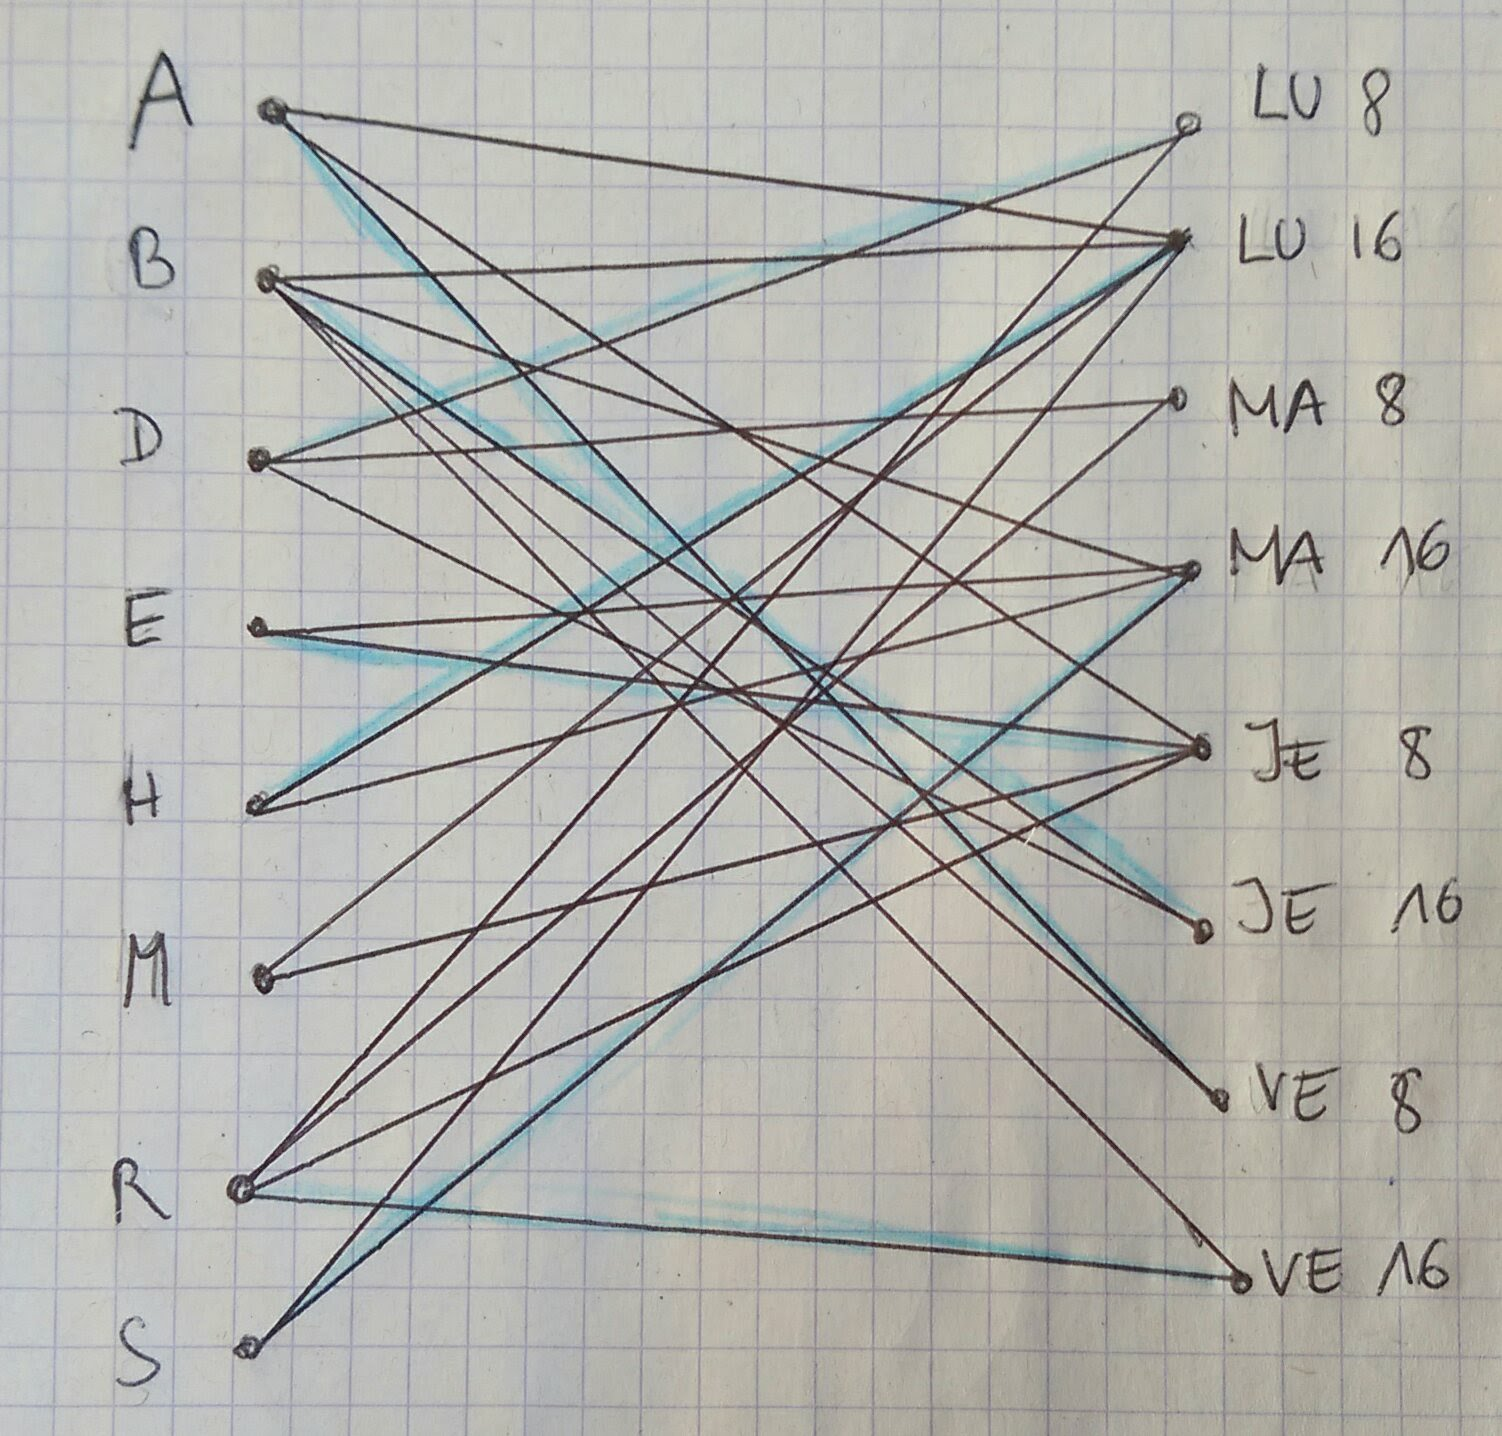
\includegraphics[width=0.7\textwidth]{IMAG0297_1.jpg}
\end{solfig}

\end{solution}

\section{Question 2}
\begin{enumerate}
	\item Démontrez que dans une suite de 5 nombres réels distincts
	se trouve une sous-suite croissante de 3 éléments,
	ou une sous-suite décroissante de 3 nombres.
	Par exemple, la suite $12, 3, 9, 7, 5$
	contient la sous-suite décroissante $12, 9, 7$.
	\item Démontrez que pour tous les naturels $r$, $s$,
	il existe un nombre fini $f(r, s)$
	tel que toute suite de $f(r, s)$ réels distincts
	contient une sous-suite croissante de $r$ éléments
	ou une sous-suite décroissante de $s$ éléments.
\end{enumerate}

\begin{solution}
	\begin{enumerate}
		\item On utilise un théorème dû à Erd\H{o}s et Szekeres,
		prouvé en 1935,
		qui dit que toute liste de plus de $n^2$ nombres distincts
		a un sous-liste monotone de longueur supérieure à $n$,
		appliquée pour $n = 2$.
		\begin{proof}
			Soit $a = a_1, \ldots, a_{n^2+1}$ la liste.
			On assigne à la position $k$ l'annotation $(x_k, y_k)$,
			où $x_k$ est la longueur de
			la plus longue sous-liste croissante
			se terminant en $a_k$,
			et $y_k$ est la longueur de
			la plus longue sous-liste décroissante
			se terminant en $a_k$.
			Si $a$ n'a pas de sous-liste monotone de longueur $n+1$,
			alors $x_k$ et $y_k$ ne dépassent jamais $n$,
			et il n'y a que $n^2$ annotations possibles.

			Comme la liste est de longueur $n^2+1$,
			le principe des tiroirs implique
			que deux annotations doivent être les mêmes.
			C'est impossible lorsque les éléments de $a$
			sont distincts.
			Quand $i < j$ et $a_i < a_j$,
			on peut concaténer la plus longue séquence croissante
			se terminant en $a_i$ et $a_j$.
			Lorsque $i < j$ et $a_i > a_j$,
			on peut concaténer la plus longue séquence décroissante
			se terminant en $a_i$ avec $a_j$.
		\end{proof}
		\item Par le même théorème
		appliqué à $n = \max\{\,r, s\,\} - 1$,
		un liste de longueur supérieure à $n^2$ sera suffisante.
		Il suffit donc de dire
		\[
		f(r, s) = n^2 + 1 = \left(\max\{\,r, s\,\} - 1 \right)^2 + 1\,.
		\]

		Une borne plus serrée
		est atteinte en utilisant une généralisation du théorème
		(également due à Erd\H{o}s et Szekeres).
		En effet, un liste de longueur $ab + 1$,
		avec des nombres distincts,
		a une sous-séquence croissante de taille $a+1$
		ou une sous-séquence décroissante de taille $b+1$.
		Dans ce cas-ci, on poserait donc
		\[
		f(r, s) = (r-1)(s-1)+1 = rs - r - s\,.
		\]
	\end{enumerate}
\end{solution}

\section{Question 3}
On sait que le nombre chromatique d’un graphe simple $G$
est borné par $\chi(G) \leq \Delta(G)+1$.

\begin{enumerate}
	\item Illustrez cette borne pour l’étoile à $n$ n\oe{}uds
	(qui est un arbre avec une racine et $n - 1$ feuilles).
	Est-ce une bonne borne, à votre avis?
	\item Démontrez que $\chi(G) \le \max_{F \subseteq G} \delta(F) + 1$,
	où $F$ est un sous-graphe $G$. (Indice: par exemple par induction.)
	\item Démontrez que cette borne est toujours
	au moins aussi la borne $\Delta(G) + 1$.
	\item Illustrez cette borne sur l'étoile à $n$ n\oe{}uds.
	\item Démontrez que pour tout graphe planaire $G$,
	on a $\max_{F \subseteq G} \delta(F) + 1 \le 6$.
	Cette borne démontre le \og théorème des 6 couleurs \fg{}.
	\item Bonus: démontrez que $\chi(G) \le \lambda + 1$
	où $\lambda$ est la plus grande valeur propre
	de la matrice d'adjacence $A$ de $G$
	(c'est un nombre réel positif,
	qu'on peut aussi caractériser comme
	$\lambda = \max_{x \in \R^{n}} \frac{x^T A x}{x^T x}$,
	de par la symétrie de $A$).
\end{enumerate}

\begin{solution}

\begin{enumerate}
	\item Avec une étoile à $6$ noeuds, $\Delta(G) = 5$,
	donc on peut utiliser $6$ couleurs.
	Cette borne est ici très mauvaise, $2$ couleurs suffisent,
	comme le graphe est biparti!
	\begin{solfig}{c}{Première sous question de la question 3.}
		\centering
		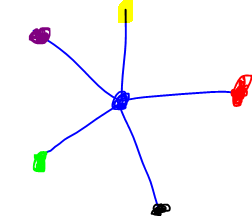
\includegraphics[scale=0.75]{jan2017MinQ3.PNG}
		\label{fig:univerise}
	\end{solfig}
	\item \nosubsolution
	\item \nosubsolution
	\item \nosubsolution
	\item Comme $G$ est un graphe planaire simple,
	tout sous-graphe $F$ de $G$ est également planaire et simple.
	On peut alors démontrer que ce graphe
	a un sommet de degré au plus $5$.
	\begin{proof}
		On montre la proposition équivalente
		que le degré moyen est plus petit que $6$.
		Si $n(G) < 3$, alors $d(v) \le n(G) - 1 < 2 < 5$
		pour tout $v \in V(G)$.
		Si $n(G) \ge 3$, on a $e(G) \le 3 n(G) - 6$.
		Le degré moyen est donné par
		\[
		\frac{\sum_{v \in V(G)} d(v)}{n(G)} = \frac{6 n(G)-12}{n(G)} < 6\,.\qedhere
		\]
	\end{proof}
	Comme le degré minimal est au plus $5$,
	l'égalité désirée est bien prouvée,
	ce qui démontre le théorème des $6$ couleurs.
	\item \nosubsolution
\end{enumerate}

\end{solution}

\section{Question 4}
Vrai ou faux.

\begin{enumerate}
	\item Tout graphe connexe à $n$ n\oe{}uds
	et $n + 1$ arêtes est planaire.

	\item Toute représentation dans le plan d’un graphe simple
	à $n \ge 3$ n\oe{}uds et $m$ arêtes
	comporte au moins $m - 3n + 6$ croisements d’arêtes.

	\item Il existe un graphe planaire qui est $6$-connexe.

	\item Tout arbre $G$ possède au moins $\Delta(G)$ feuilles.

	\item Si je dispose $120$ pièces de $1$ euro à plat sur la table,
	éventuellement contigües,
	je peux en trouver $30$ non contigües deux à deux.

\end{enumerate}

\begin{solution}

\begin{enumerate}
	\item VRAI. Pour que le graphe soit connexe,
	on doit utiliser $n-1$ arêtes,
	il en reste $2$.
	Donc, c'est impossible d'obtenir $K_5$ ou $K_{3,3}$
	en rajoutant seulement $2$ arêtes à une chaine;
	c'est un graphe planaire.

	\item VRAI. % TODO proof

	\item FAUX. Tout graphe $6$-connexe contient $K_6$, qui contient $K_5$.
	Par le Théorème de Kuratowski, le graphe n'est alors pas planaire.

	\item VRAI. % TODO proof

	\item VRAI. Tout graphe planaire possède un coloriage propre
	de $4$ couleurs,
	alors il existe d'office un ensemble indépendant
	d'au moins $30$ pièces,
	car la somme des quatre ensembles indépendants doit être égale à $120$.

\end{enumerate}

\end{solution}

\end{document}
